\chapter{Project Time Management}
The project timeline is divided into the product's development sections and the mandatory meetings and deadlines provided by the customer. The different development phases and deadlines can be seen in the Gantt diagram of the project timeline \ref{fig:gantt_timeline}.

\begin{figure}[h]
    \centering
    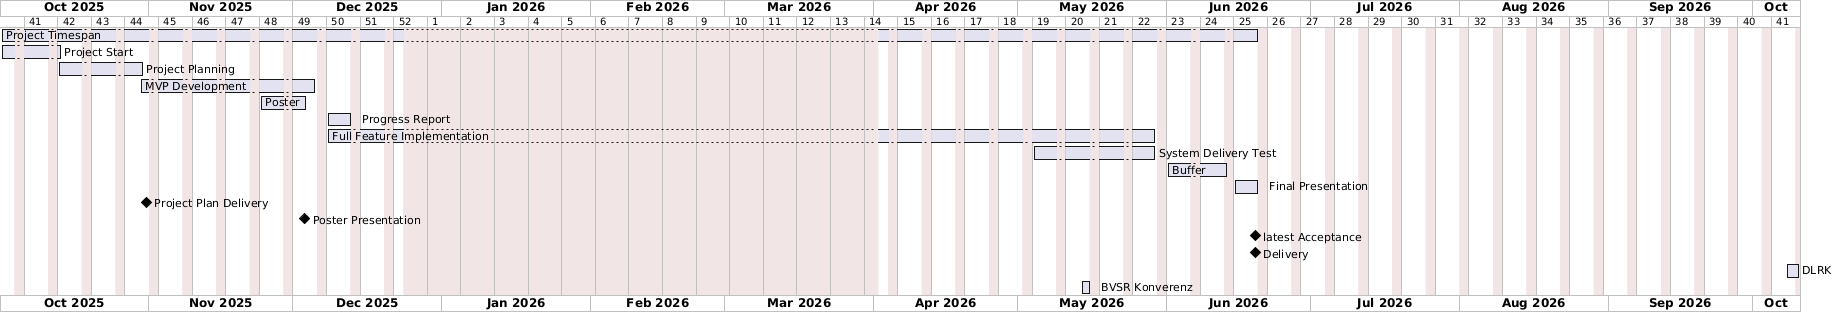
\includegraphics[width=1.0\linewidth]{img/project_plan_gantt_v2.png}
    \caption{Gantt Timeline}
    \label{fig:gantt_timeline}
\end{figure}

\section{Timeline}
As can be seen in the Gantt diagram, the project has a total length of 38 weeks, of which 24 weeks or 120 days are available for development. These available development days are grouped into phases. These will now be explained in detail.

\subsection{Project Planning}
During this phase, the team meets to review the tasks involved in the project. The project development plan and other key documents are also written during this phase. Only high-level requirements are written on the technical side.

\subsection{Minimum Viable Product (MVP) Development}
In this phase, the team will begin developing critical systems and functionality. The goal is not to develop the complete scope of the product, but rather to create something that can be presented to users and demonstrate that the team's decisions are functioning as intended. If the customer has any changes they would like to make, they can be incorporated at this point without causing any major delays.

\subsection{Poster}
During this phase, the team creates the poster to be displayed at the poster session. This phase runs in parallel with the development process and is not directly tied to any progress made during this process.

\subsection{Progress Report}
During this phase, the team will meet with the customer to discuss whether the work completed so far meets their standards and expectations. Changes to the project scope are still possible at this stage, but depending on the change request, they may result in a significant time penalty.

\subsection{Full Feature Implementation}
In this phase, the team will develop the full feature set that was not implemented in the MVP phase. Changes to the scope or architecture at this stage will incur significant time penalties, which will most likely result in missed deadlines or project failure.

\subsection{System Delivery Test}
In this phase, the product is tested against the customer specifications and high-level requirements, according to the development process model. Lower-level tests and unit tests are carried out in parallel with the implementation of individual features and are therefore not listed in this timeline.

\subsection{Buffer}
The purpose of this phase is to act as a buffer, ensuring that missed deadlines or human error during the development phase do not impact the project delivery deadline.

\subsection{Final Presentation}
During this phase, the final product is presented to the customer for review. The date of this presentation is determined by the customer, who must give the development team at least two weeks' notice. If the customer does not provide a date for the final presentation, the development team will assume that it will occur on the last day of this phase.

\section{Deadlines}
The following sections describe the various deadlines relevant to the development team. These deadlines do not include those outside the project scope, such as the BVSR conference and the Deutscher Luft- und Raumfahrtkongress (DLRK).

\subsection{Project Plan Delivery}
By this deadline, the team will provide the project plan that was created during the planning phase. Any changes to the scope or features after this date will result in the generation of a new version of the project plan.

\subsection{Poster Presentation}
By this deadline, the team will present the poster created during the project poster phase. The deadline for deciding what can be included in the poster must be set before the poster phase begins.

\subsection{Latest Acceptance}
This deadline marks the latest time the customer will accept the project. The customer is expected to judge the project based on the most recent version of the agreed project plan document.

\subsection{Delivery}
This deadline marks the date by which the project must be completed. It also marks the end of the official project period. However, other work, such as writing a paper, can continue after this date.

\subsection{Other Phases and Deadlines}
The team intends to write a paper about the project's implementation. The timeline for writing and submitting the paper will be announced at a later date.
